% =====================================================================
% A single renormalized energy denominator controls the nonperturbative
% loop expansion of quantum spin ice.
%
% Supersedes paper_A_selection_rules, paper_B_material_verdict and
% paper_C_emergent_maxwell (archived).  Numbers marked \pending{} are not
% yet computed; everything else is traced in README.md.
% =====================================================================
\documentclass[aps,prb,preprint,amsmath,amssymb,superscriptaddress,
longbibliography,floatfix]{revtex4-2}

\usepackage{bm}
\usepackage{graphicx}
\usepackage{xcolor}
\usepackage[colorlinks=true,citecolor=blue!55!black,
urlcolor=blue!55!black,linkcolor=blue!55!black]{hyperref}
\graphicspath{{figs/}}
\setlength{\emergencystretch}{3em}

\newcommand{\Jzz}{J_{zz}}
\newcommand{\Jpm}{J_{\pm}}
\newcommand{\Deff}{D_{\rm eff}}
\newcommand{\pending}[1]{{\color{red}\textbf{[PENDING: #1]}}}

\begin{document}

\title{A single renormalized energy denominator controls the\\
nonperturbative loop expansion of quantum spin ice}

\author{Zhengbang Zhou}
\email{zhengbang.zhou@mail.utoronto.ca}
\affiliation{Department of Physics, University of Toronto, Toronto,
Ontario M5S 1A7, Canada}

\author{Yong Baek Kim}
\email{ybkim@physics.utoronto.ca}
\affiliation{Department of Physics, University of Toronto, Toronto,
Ontario M5S 1A7, Canada}

\date{\today}

\begin{abstract}
The low-energy theory of quantum spin ice is a loop expansion: an alternating
flip of $L$ spins around a closed path enters the ice-manifold Hamiltonian with
amplitude $K_L^{(0)}=2\binom{L-2}{L/2-1}|\Jpm|^{L/2}/\Jzz^{L/2-1}$, built from
$L/2-1$ energy denominators each taken to be $\Jzz$.  We measure these
amplitudes nonperturbatively, on finite clusters from which the noncontractible
torus processes have been removed exactly, and find that the entire
nonperturbative content is a single number.  Writing $\mu\equiv\Jzz/\Deff$, the
measured amplitudes obey $K_L=K_L^{(0)}\mu^{L/2-1}$ for $L=8,10,12$ with a
spread of $1$--$3.5\%$ across the whole coupling range and two virtual depths:
\emph{every} denominator is renormalized from $\Jzz$ to a common
$\Deff(\Jpm)$.  Two exact sum rules make $\Deff$ well defined rather than
fitted --- the second-order amplitude vanishes identically and the first
spectral moment is exactly $12|\Jpm|^3$ --- so that $\Deff=\sqrt{M_1/K_6}$
equals $\Jzz$ in leading perturbation theory by construction.  We measure
$\Deff/\Jzz=1.17\rightarrow3.35$ over $|\Jpm|/\Jzz=0.03\rightarrow0.30$, and
verify that it is intensive: doubling the cluster from $16$ to $32$ sites moves
it by less than $10\%$.  The hexagon amplitude is therefore suppressed by
$\mu^2$, a factor of $11$ at $|\Jpm|/\Jzz=0.30$ and $4.3$ at the couplings
relevant to the cerium pyrochlores.  Three consequences follow.  The emergent
photon scale is several times colder than the standard estimate.  The two
peaks of the specific heat do not merge: the perturbative ratio grows as
$|\Jpm|^3$ but $\mu^2$ falls faster, and the merging seen both in perturbation
theory and in naive periodic exact diagonalization is an artifact.  For
$\rm Ce_2Hf_2O_7$ and $\rm Ce_2Zr_2O_7$ the gauge feature lies at a few mK,
below every temperature yet measured, so a single broad hump is the expected
signature rather than evidence for large transverse exchange.  We identify the
entropy released below the observed hump, which must be
$\tfrac{R}{2}\ln\tfrac32$, as the parameter-free measurement that decides
between these readings.
\end{abstract}

\maketitle

\section{Introduction}
\label{sec:intro}

Quantum spin ice (QSI) is the three-dimensional compact $U(1)$ lattice gauge
theory realized by a spin-$1/2$ pyrochlore magnet with dominant Ising exchange
~\cite{Hermele2004,Gingras2014,Benton2012,RauGingras2019}.  Its standard
derivation restricts the Hilbert space to the two-in--two-out ice manifold and
generates, at third order in the transverse exchange, a ring-exchange term
around each hexagon.  Every quantitative statement about the emergent photon
--- its speed, its bandwidth, the temperature of the thermodynamic crossover
into the gauge sector --- is anchored on the coefficient of that term,
\begin{equation}
 g_6=\frac{12|\Jpm|^3}{\Jzz^2}.
 \label{eq:g6}
\end{equation}
The derivation is controlled at small $|\Jpm|/\Jzz$.  The materials are not:
the cerium pyrochlores sit near $|\Jpm|/\Jzz\simeq0.13$--$0.16$, where the
third-order truncation is an assumption rather than a limit.

This paper measures the loop amplitudes directly instead of assuming them.  The
measurement is possible because two obstructions have been removed.  The first
is topological: a periodic cluster is a torus, and supports ice-preserving spin
rearrangements that close only through a periodic image, entering at order
$\Jpm^2$ --- one order \emph{before} the physical hexagon --- and manufacturing
the dominant low-energy scale~\cite{ZhouKimMask}.  We work throughout with the
transport-masked map of Ref.~\cite{ZhouKimMask}, in which those processes are
deleted exactly.  The second is that a nonperturbative amplitude must be
compared with perturbation theory on equal terms; Sec.~\ref{sec:deff}
establishes two exact sum rules that fix the comparison with no fitted
quantity.

The result is that the nonperturbative loop expansion has the same form as the
perturbative one, with one number changed.  Section~\ref{sec:collapse} reports
the collapse; Sec.~\ref{sec:deff} makes it exact; Sec.~\ref{sec:origin} asks
where the renormalization comes from; Sec.~\ref{sec:consequences} works out
what it does to the emergent photon, to the two-peak specific heat, and to the
two materials in which these questions are currently being asked.

\section{Model, cluster and mask}
\label{sec:model}

We study the nearest-neighbour XXZ model on the pyrochlore lattice,
\begin{equation}
 H=H_0+V,\qquad
 H_0=\Jzz\sum_t\tfrac12 Q_t^2,\qquad
 V=-\Jpm\!\!\sum_{\langle ij\rangle}\!\left(S_i^+S_j^-+\mathrm{h.c.}\right),
 \label{eq:model}
\end{equation}
with $\Jzz>0$ and $Q_t=\sum_{i\in t}S_i^z$.  $P$ projects onto the ice manifold
($Q_t=0$ for all $t$), $Q=1-P$.  Energies are in units of $\Jzz$ and
$x\equiv|\Jpm|/\Jzz$.

Two clusters are used.  The $16$-site conventional cubic cell (cubic-16, $90$
ice states) is small enough that the complete virtual space is affordable, so
every quantity there is exact.  The $32$-site face-centred-cubic cluster
(FCC-32, $2970$ ice states) is the only cluster on which simple loops of
perimeter $8$, $10$ and $12$ survive at all: on cubic-16 every such loop wraps
the periodic box and is removed by the mask.  On FCC-32 the virtual space is
truncated to states within $\ell$ transverse exchanges of the ice manifold
($1.4\times10^5$, $2.5\times10^6$ and $2.2\times10^7$ states for
$\ell=1,2,3$).  Depth is a convergence parameter, unrelated to the loop
perimeter $L$.

The winding-free ice-block map is the transport mask applied to the exact
Feshbach map,
\begin{equation}
 F(z)=PHP+PVQ\,(z-QHQ)^{-1}\,QVP ,
 \label{eq:feshbach}
\end{equation}
with every matrix element connecting different covering-lattice transport
sectors deleted~\cite{ZhouKimMask}.  Since $PHP$ is diagonal on the ice
manifold, all loop amplitudes live in the second term.

\section{The loop amplitudes collapse onto one parameter}
\label{sec:collapse}

Each surviving off-diagonal element of the masked map flips the spins on which
two ice configurations differ.  Following Ref.~\cite{ZhouKimMask} we retain
only \emph{simple} loops --- the induced nearest-neighbour subgraph is
connected and every vertex has degree exactly two, which excludes products of
shorter rings joined at a vertex --- and define $K_L$ as the mean modulus of
those elements at perimeter $L$.

\begin{figure*}[t]
\centering
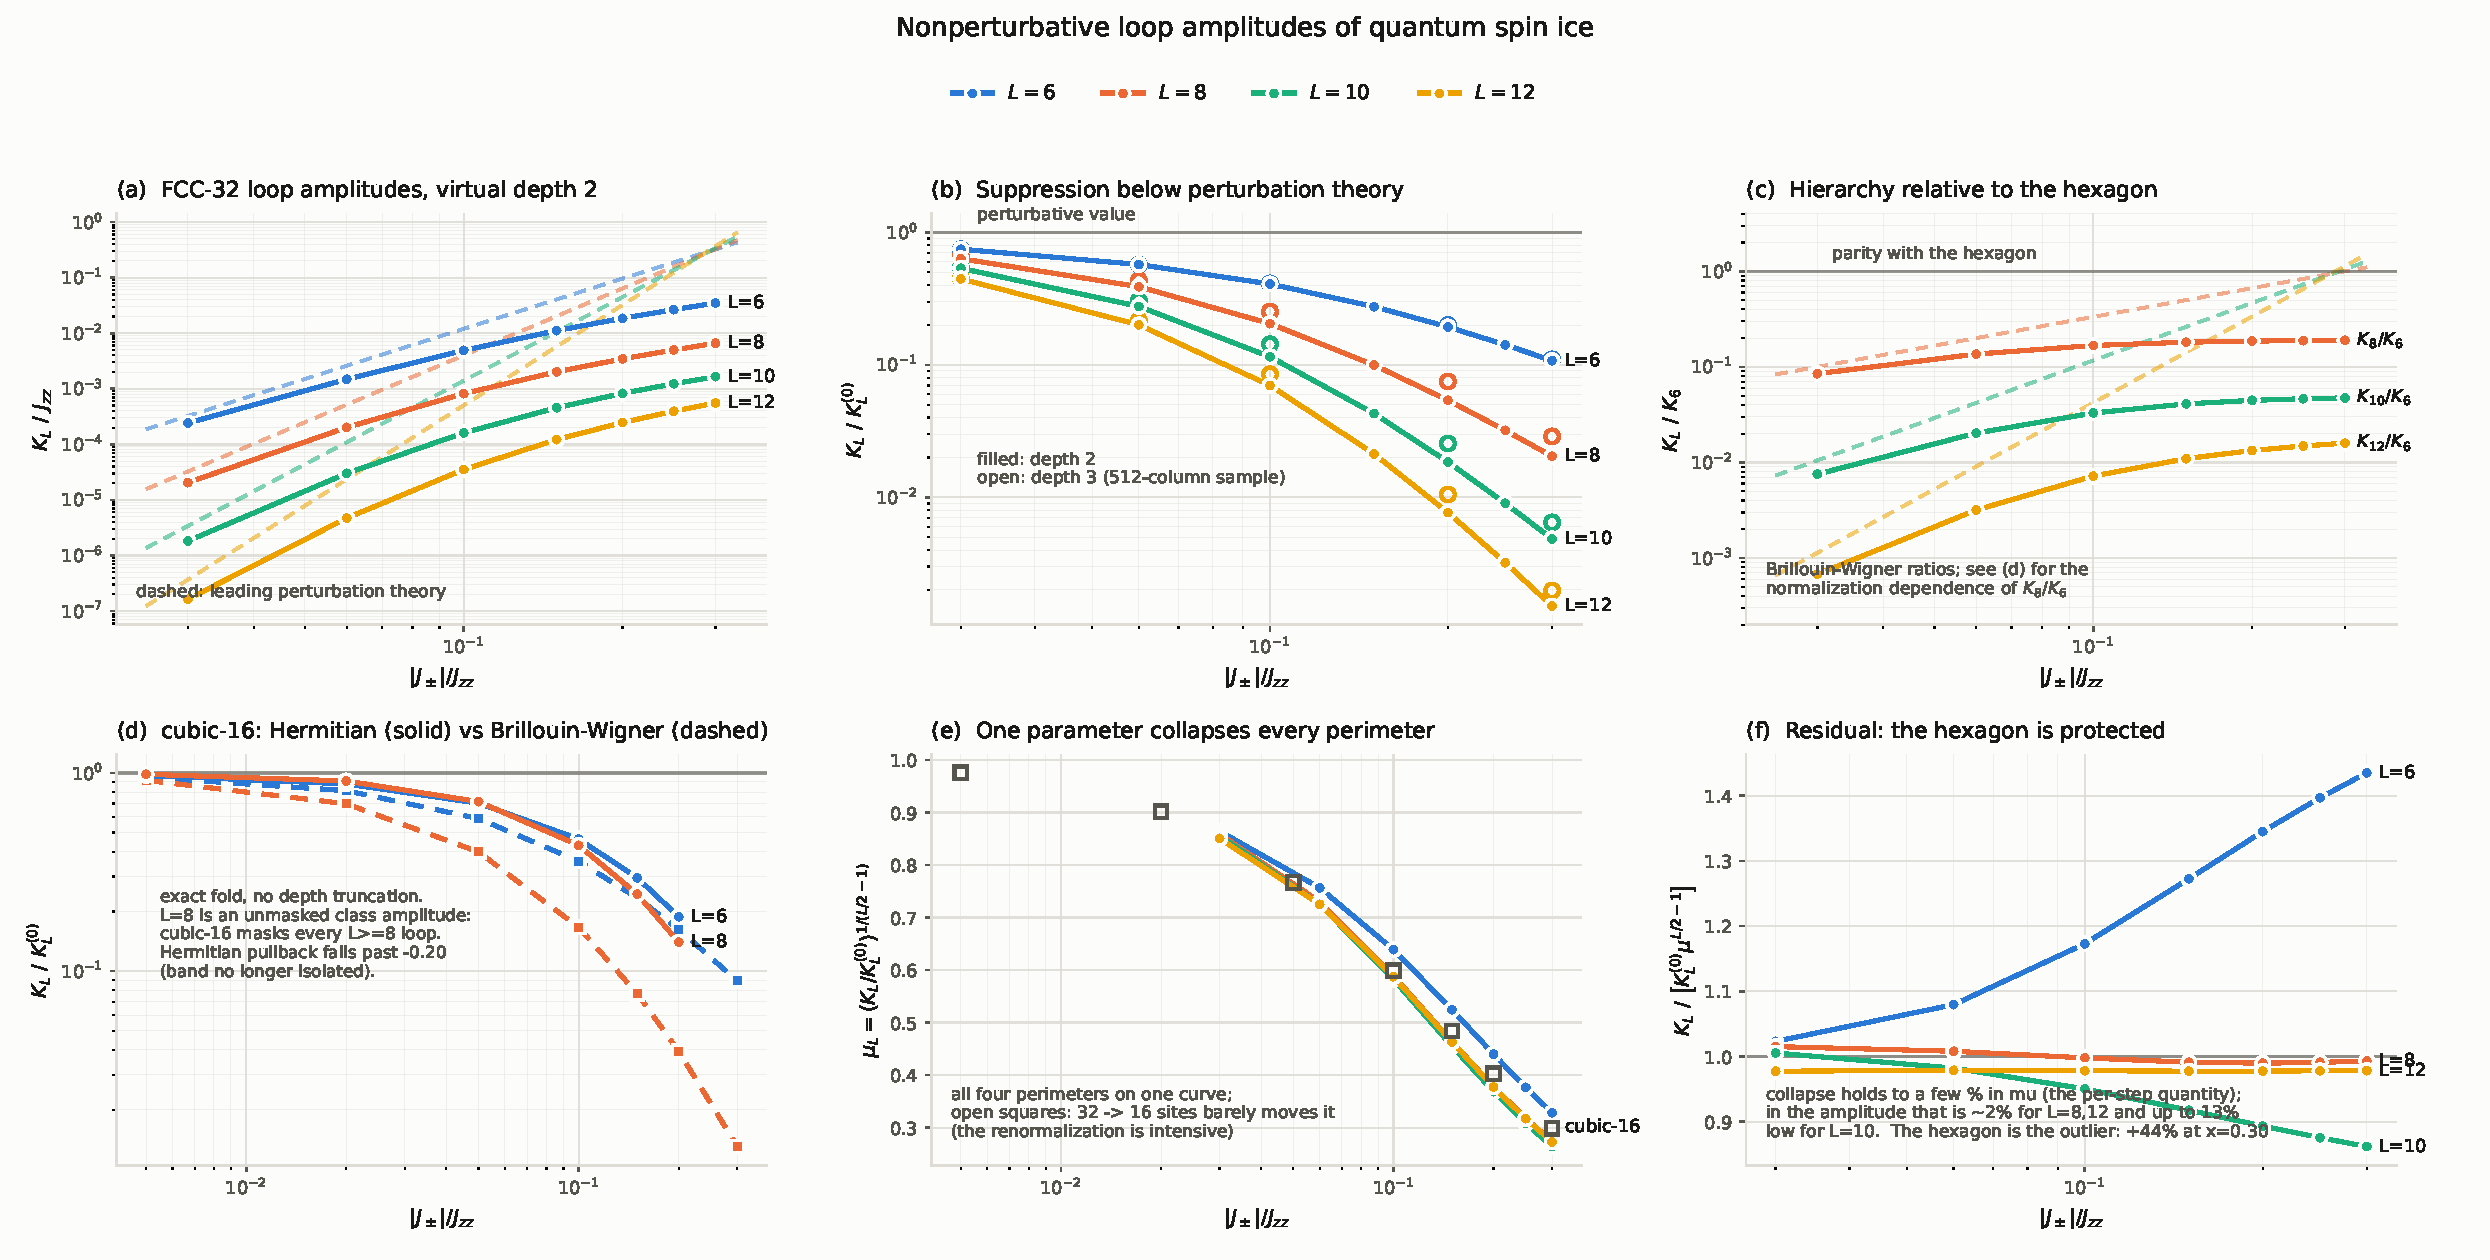
\includegraphics[width=\textwidth]{fig_loop_amplitudes.pdf}
\caption{Nonperturbative loop amplitudes on FCC-32.  (a) $K_L$ against
coupling with the leading perturbative power laws (dashed); the measured
amplitudes fall progressively below them and never cross, although the
perturbative curves do near $x=0.3$.  (b) The suppression $K_L/K_L^{(0)}$;
open symbols are matched virtual-depth-$3$ checks and lie systematically above
the depth-$2$ points, so the plotted suppression is a lower bound.  (c) The
hierarchy relative to the hexagon saturates rather than growing.  (d) cubic-16
with the exact fold: the Hermitian (des Cloizeaux) and Brillouin--Wigner
normalizations agree at weak coupling and separate at strong coupling, far more
for $L=8$ than for $L=6$.  (e) The collapse: $\mu_L=(K_L/K_L^{(0)})^{1/(L/2-1)}$
for all four perimeters, with cubic-16 as open squares.  (f) Residual of the
one-parameter law; the hexagon is the single outlier.}
\label{fig:loops}
\end{figure*}

Leading perturbation theory gives, for an alternating simple loop of perimeter
$L=2n$ completed by $n$ exchanges,
\begin{equation}
 K_L^{(0)}=2\binom{L-2}{L/2-1}\frac{|\Jpm|^{L/2}}{\Jzz^{L/2-1}} ,
 \label{eq:KL0}
\end{equation}
i.e.\ $12$, $40$, $140$ and $504$ for $L=6,8,10,12$.  The structure that
matters below is that Eq.~(\ref{eq:KL0}) contains $n-1=L/2-1$ energy
denominators, each set to $\Jzz$.

We therefore test the hypothesis that the entire nonperturbative effect is a
common renormalization $\mu$ of each denominator,
\begin{equation}
 \boxed{\;K_L=K_L^{(0)}\,\mu^{\,L/2-1}\;}
 \label{eq:collapse}
\end{equation}
with one $\mu$ per coupling and no per-perimeter freedom.  Extracting
$\mu_L=(K_L/K_L^{(0)})^{1/(L/2-1)}$ separately for each perimeter tests it
without fitting anything:

\begin{table}[b]
\caption{FCC-32, virtual depth $2$.  Three independent perimeters spanning two
decades in amplitude agree on one number.  The $L=6$ column is shown for
contrast and is discussed in the text.}
\label{tab:collapse}
\begin{ruledtabular}
\begin{tabular}{cccccc}
$x$ & $\mu_6$ & $\mu_8$ & $\mu_{10}$ & $\mu_{12}$ & spread ($L\ge8$)\\ \hline
0.03 & 0.8646 & 0.8590 & 0.8559 & 0.8508 & $1.0\%$\\
0.06 & 0.7567 & 0.7302 & 0.7250 & 0.7252 & $0.7\%$\\
0.10 & 0.6390 & 0.5896 & 0.5826 & 0.5874 & $1.2\%$\\
0.15 & 0.5246 & 0.4637 & 0.4552 & 0.4630 & $1.8\%$\\
0.20 & 0.4398 & 0.3780 & 0.3687 & 0.3776 & $2.5\%$\\
0.25 & 0.3765 & 0.3176 & 0.3082 & 0.3172 & $3.0\%$\\
0.30 & 0.3282 & 0.2734 & 0.2640 & 0.2728 & $3.5\%$\\
\end{tabular}
\end{ruledtabular}
\end{table}

Equation~(\ref{eq:collapse}) holds to a few percent over the full range, and
the same collapse is obtained independently at virtual depth $3$.
Figure~\ref{fig:loops}(e) shows it directly.  The hexagon is the one
systematic outlier, lying above the common law by $1\%$ at $x=0.03$ rising to
$21\%$ in $\mu$ (equivalently $44\%$ in the amplitude) at $x=0.30$: the
shortest loop is slightly protected relative to the universal law obeyed by the
longer ones.

Two immediate corollaries.  First, the saturation of the hierarchy in
Fig.~\ref{fig:loops}(c) is not new physics: Eq.~(\ref{eq:collapse}) gives
\begin{equation}
 \frac{K_{L+2}}{K_L}=\left(4-\frac4L\right)x\,\mu(x) ,
 \label{eq:ratio}
\end{equation}
and $x\mu(x)$ saturates ($0.026\rightarrow0.082$ from $x=0.03$ to $0.30$), so
the perturbative linear growth is cancelled by the fall of $\mu$.  At $x=0.30$
this predicts $K_{10}/K_8=0.288$ against $0.250$ measured.  Second, the
expansion remains local in perimeter: $K_8/K_6\rightarrow0.19$,
$K_{10}/K_6\rightarrow0.047$, $K_{12}/K_6\rightarrow0.016$.

\section{The renormalized denominator is exactly defined}
\label{sec:deff}

Equation~(\ref{eq:collapse}) invites the reading that each perturbative
denominator $\Jzz$ is replaced by some $\Deff=\Jzz/\mu$.  That reading can be
made exact rather than interpretive, using two sum rules.

Decompose the second term of Eq.~(\ref{eq:feshbach}) over the eigenstates of
the \emph{full} $QHQ$, $QHQ|k\rangle=E_k|k\rangle$.  For two ice states $a,b$
related by one contractible hexagon, define
\begin{equation}
 w_k=\langle b|PVQ|k\rangle\langle k|QVP|a\rangle,\qquad
 M_n=\sum_k w_kE_k^{\,n}=\langle b|VQ(QHQ)^nQV|a\rangle .
 \label{eq:moments}
\end{equation}
The amplitude at the physical anchor $z_0$ (the ground energy of the same
truncated microscopic Hamiltonian) is $K_6=\sum_k w_k/(z_0-E_k)$.  Two facts,
both verified numerically to machine precision on both clusters and at every
coupling:
\begin{align}
 M_0&=\langle b|VQV|a\rangle=0,
 \label{eq:M0}\\
 M_1&=\langle b|VQVQV|a\rangle=12|\Jpm|^3 .
 \label{eq:M1}
\end{align}
Equation~(\ref{eq:M0}) is a selection rule: two applications of $V$ move at
most four spins, while a hexagon pair differs by six.  Equation~(\ref{eq:M1})
states that the first spectral moment is exactly the third-order
\emph{numerator} of Eq.~(\ref{eq:g6}), with no denominators.  Note the
reorganization relative to textbook perturbation theory: one denominator is
explicit in the resolvent, and the second is carried by the eigenvectors of
$QHQ$, which contain $V$.

Define
\begin{equation}
 \Deff\equiv\sqrt{M_1/K_6} .
 \label{eq:Deff}
\end{equation}
This is a definition, but Eqs.~(\ref{eq:M0}) and (\ref{eq:M1}) fix its content:
in leading perturbation theory $K_6\rightarrow g_6=12|\Jpm|^3/\Jzz^2$ while
$M_1=12|\Jpm|^3$, so $\Deff=\Jzz$ \emph{exactly}.  $\Deff$ is therefore the
effective value of the product of the two perturbative denominators, and
\begin{equation}
 \frac{K_6}{g_6}=\left(\frac{\Jzz}{\Deff}\right)^2=\mu^2 .
 \label{eq:mudef}
\end{equation}
Because $\sum_kw_k=0$, the amplitude is not a sum of same-sign contributions:
had all intermediate states been degenerate, $K_6$ would vanish identically.
The amplitude is generated by the variation of $(E_k-z_0)^{-1}$ across the
intermediate spectrum, and $\Deff$ is a weighted mean of $E_k-z_0$, not the
energy of any single state.

\begin{figure*}[t]
\centering
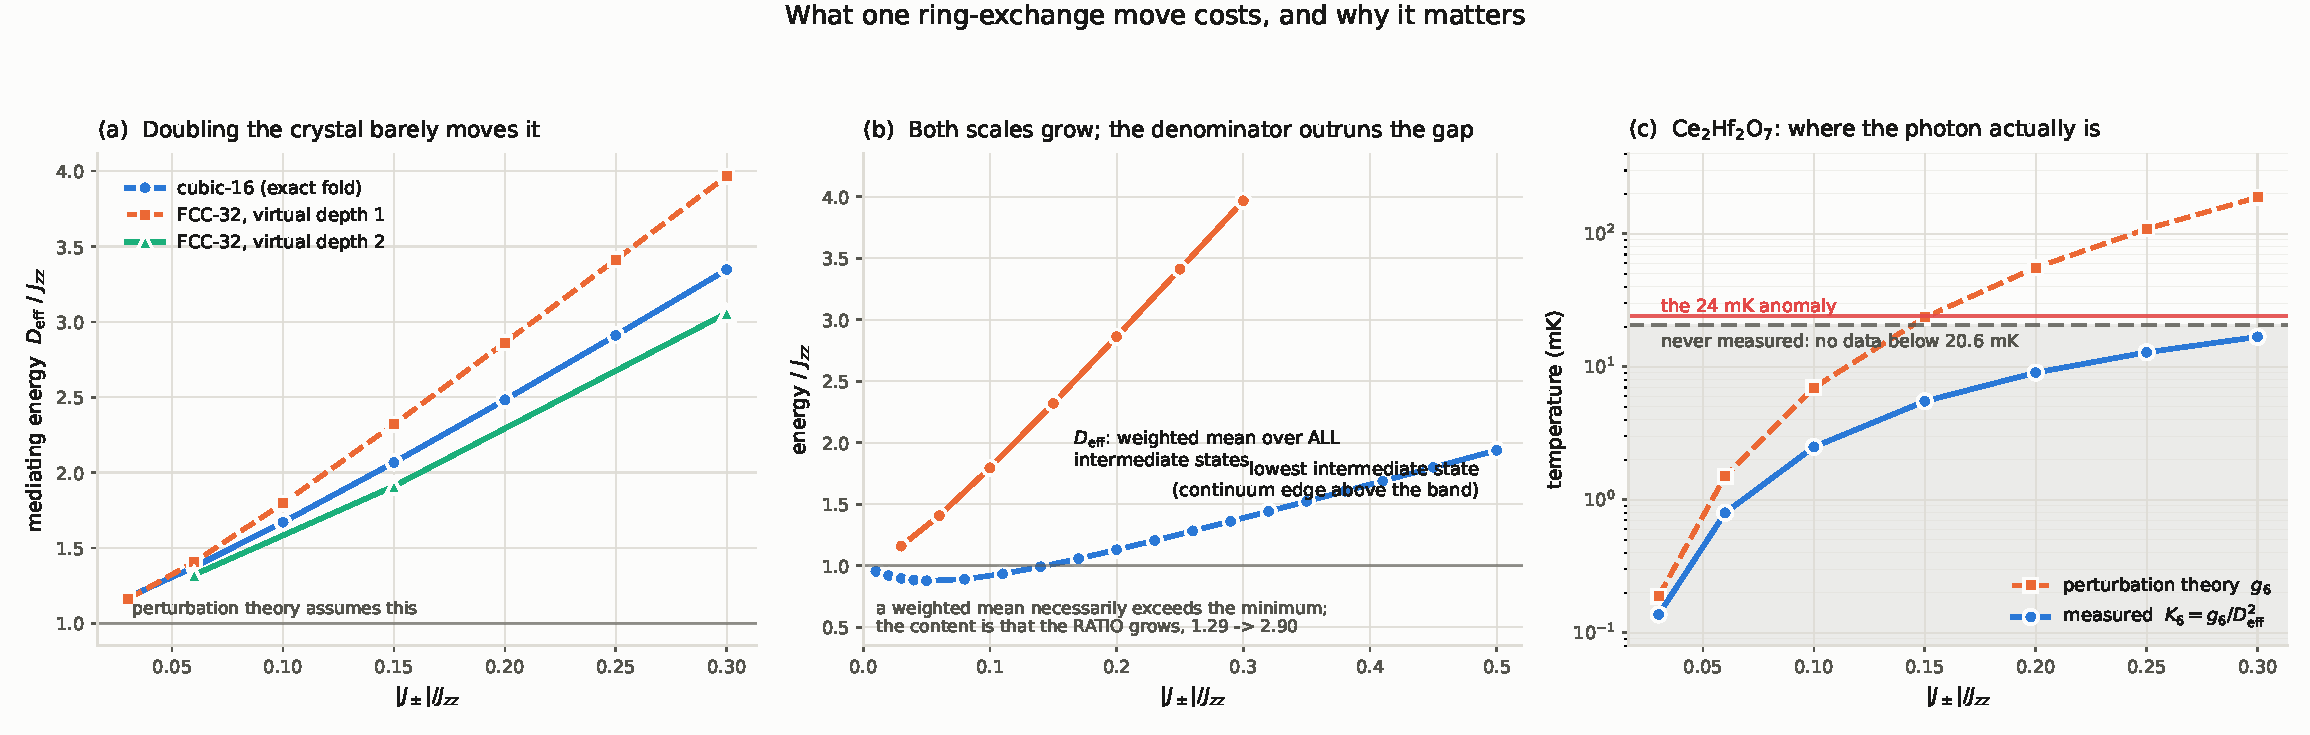
\includegraphics[width=\textwidth]{fig_denominator.pdf}
\caption{(a) $\Deff$ is intensive: cubic-16 with the complete virtual space
and FCC-32 at two virtual depths agree to under $10\%$ at matched depth,
against the factor of two an extensive quantity would give.  Perturbation
theory is the line at $1$.  (b) $\Deff$ against the lowest intermediate-state
energy (continuum edge above the ice band).  A weighted mean necessarily
exceeds a minimum; the content is that the ratio grows, from $1.29$ to $2.90$.
(c) The consequence in physical units for $\rm Ce_2Hf_2O_7$
($\Jzz=0.050$~meV): the perturbative estimate crosses the observed $24$~mK
anomaly at exactly the fitted couplings, whereas the measured amplitude never
reaches the coldest temperature yet measured on the material.}
\label{fig:denominator}
\end{figure*}

\subsection{Two controls}

\emph{Intensivity.}  $\Deff$ is a difference of two absolute energies, so it is
an excitation energy and should not scale with volume.  Measured on the
hexagon channel [Fig.~\ref{fig:denominator}(a)], cubic-16 with the exact fold
gives $\Deff/\Jzz=1.374$, $2.067$, $3.346$ at $x=0.06,0.15,0.30$, against
$1.322$, $1.910$, $3.058$ on FCC-32 at depth $2$ --- ratios $0.962$, $0.924$,
$0.914$.  Doubling the number of sites moves $\Deff$ by less than $10\%$.  The
suppression is a local property of the theory, not a finite-volume or
Brillouin--Wigner size-inconsistency artifact.

\emph{Normalization.}  $F(z)$ is a Brillouin--Wigner map: energy dependent, and
not a Hermitian effective Hamiltonian.  We therefore repeat the hexagon
measurement using the Hermitian des Cloizeaux (L\"owdin polar) pullback of the
exact band onto the ice manifold, which is residue free.  On cubic-16 the two
normalizations agree at weak coupling, $K_6/g_6=0.952$ (BW) against $0.971$
(Hermitian) at $x=0.005$, confirming that the comparison with
Eq.~(\ref{eq:g6}) is properly calibrated, and separate mildly at stronger
coupling: $0.234$ against $0.296$ at $x=0.15$, and $0.162$ against $0.188$ at
$x=0.20$.  The correction to $\mu$ peaks near $1.29$ and does \emph{not} track
$1/Z$, so the residue is not driving the effect.  The correction is, however,
strongly perimeter dependent --- at $x=0.20$ it is $1.16$ for $L=6$ but $3.56$
for $L=8$ [Fig.~\ref{fig:loops}(d)] --- so the ratios $K_L/K_6$ are
normalization sensitive at the tens-of-percent level even though $\mu$ itself
is not.  Beyond $x\simeq0.20$ the ice-descended band ceases to be isolated on
cubic-16 and the Hermitian object does not exist.

\section{Where the renormalization comes from}
\label{sec:origin}

$\Deff$ rises from $1.17\,\Jzz$ to $3.35\,\Jzz$ across the range studied.  Since
$\Deff$ is a weighted mean of $E_k-z_0$, the growth means that distribution
shifts upward.  The decomposition is visible in the spectrum itself: between
$x=0.01$ and $x=0.50$ the bottom of the masked ice band falls from $-0.006$ to
$-3.558$, whereas the continuum edge falls only from $0.948$ to $-1.620$, so
the gap between them grows from $0.954$ to $1.939$.  The ice manifold is
stabilized faster than the states above it, and every excitation energy
$E_k-z_0$ grows accordingly.

Leading perturbation theory uses unperturbed energies in both places; the exact
map uses the true $z_0$ and the dressed $E_k$.  The difference between the two
is the entire effect, and it is the resummation of the higher-order processes
that flip the same six spins.  We stress what is \emph{not} being claimed:
longer loops are distinct operators acting on different spin sets and cannot
renormalize $K_6$.  The nontrivial content of Sec.~\ref{sec:collapse} is that
the same $\mu$ governs both the correction to the hexagon coefficient and the
coefficients of those independent longer-loop operators.

The physical reading --- that the ring exchange stabilizes the manifold it acts
on and thereby raises its own energy denominator, a self-limiting feedback ---
is an interpretation of the ordering above, not an independent measurement.

\section{Consequences}
\label{sec:consequences}

\subsection{The emergent photon is colder than the standard estimate}

The physical ring-exchange coupling is $K_6=g_6\mu^2$.  At the couplings
relevant to the cerium pyrochlores this is a suppression of $4.3$
($x=0.15$), and it reaches $11$ at $x=0.30$.  Every quantity anchored on $g_6$
inherits the factor: the photon bandwidth, the emergent speed of light, the
$T^3$ coefficient of the low-temperature specific heat, and the temperature of
the gauge crossover.

\subsection{The two specific-heat peaks do not merge}

The standard reading of a single broad hump in a QSI candidate is that the
transverse exchange is large enough that the gauge and spinon features have
merged.  That reading rests on Eq.~(\ref{eq:g6}): with the spinon scale
$\simeq0.25\Jzz$ roughly fixed, the ratio $T_{\rm gauge}/T_{\rm spinon}\simeq
48x^3$ reaches unity near $x\simeq0.28$.  Two independent corrections remove
the mechanism.

First, the ratio is $48x^3\mu(x)^2$, and since $\mu\simeq(1+ax)^{-1}$ with
$a\approx8$, the cubic growth that drives the merge becomes \emph{linear} at
large $x$.  Merging would require $x\sim a^2/48\approx1$, i.e.\
$|\Jpm|\sim\Jzz$, far outside any spin ice.

Second, the merging is directly observable as a torus artifact.  On cubic-16,
comparing the naive periodic full spectrum with the winding-free one at the
same coupling:
\begin{center}
\begin{tabular}{ccc}
$x$ & periodic peaks & winding-free peaks\\ \hline
$0.20$ & $0.1006,\ 0.2418$ & $0.0060,\ 0.0275,\ 0.348$\\
$0.30$ & $0.1634$ (one) & $0.0056,\ 0.0419,\ 0.460$\\
$0.45$ & $0.2162$ (one) & $0.0120,\ 0.1190,\ 0.592$\\
$0.50$ & $0.2308$ (one) & $0.0608,\ 0.1282,\ 0.632$\\
\end{tabular}
\end{center}
The periodic calculation merges at $x\ge0.30$ exactly as the standard picture
predicts; the winding-free calculation on the same cluster never does.  We note
that the periodic two-peak ratio at $x=0.20$ is $0.416$, close to the value
measured in $\rm Ce_2Hf_2O_7$ --- so a small periodic cluster reproduces the
observed ratio through the artifact.

\subsection{The cerium pyrochlores}

Taking $\Jzz=0.050$~meV $=580$~mK, the two estimates of the gauge scale are

\begin{center}
\begin{tabular}{cccccc}
$x$ & 0.10 & 0.15 & 0.20 & 0.25 & 0.30\\ \hline
$g_6$ (mK) & 6.96 & 23.50 & 55.70 & 108.8 & 188.0\\
$K_6$ (mK) & 2.50 & 5.50 & 9.04 & 12.85 & 16.79\\
\end{tabular}
\end{center}

The perturbative curve crosses the measured $24.2$~mK anomaly of
$\rm Ce_2Hf_2O_7$~\cite{Smith2025} at $x\simeq0.15$, which is where the
material is fitted --- so $g_6$ appears to explain the anomaly.  The measured
amplitude is several times smaller and does not reach $24$~mK anywhere in the
range studied; reproducing the anomaly would require $x\approx0.42$, where the
masked hexagon flux on cubic-16 has already fallen to zero and the
ice-descended band is no longer isolated.

More usefully, the published data begin at $20.6$~mK, and $K_6$ lies below that
floor for every coupling in the plausible range.  \textbf{The gauge feature has
never been inside the measured window.}  A single broad hump, as reported for
$\rm Ce_2Zr_2O_7$~\cite{Gao2019,Gaudet2019,Bhardwaj2022}, is therefore the
expected appearance of a quantum spin ice at accessible temperatures --- the
observed feature is the spinon and ice-rule crossover, with the gauge feature
an order of magnitude colder --- and its absence is not evidence against a QSI
ground state.

\section{The measurement that decides it}
\label{sec:experiment}

The merged and unmerged readings of a single hump make opposite,
parameter-free predictions for the entropy.  If the low-temperature feature is
the ordering of the ice manifold, it must release the residual ice
entropy~\cite{Pauling1935,Ramirez1999}
\begin{equation}
 S_{\rm ice}=\frac{R}{2}\ln\frac32=1.687\ \mathrm{J\,mol^{-1}K^{-1}}
 =0.293\,R\ln2 .
 \label{eq:pauling}
\end{equation}
If the peaks have merged, the observed hump contains both crossovers and
carries the full $R\ln2=5.763$~J\,mol$^{-1}$K$^{-1}$.  If they have not, the
hump carries only $0.71\,R\ln2=4.08$~J\,mol$^{-1}$K$^{-1}$ and
Eq.~(\ref{eq:pauling}) is still missing, waiting at a few mK.  No Hamiltonian,
fit or cluster enters this test.

Below the gauge crossover the specific heat of two transverse photon
polarizations must be $C\propto(k_BT/\hbar c)^3$~\cite{Benton2012}, with $c$
fixed by $K_6$ rather than $g_6$ --- a second, independent signature in the
same temperature window, and one that distinguishes the photon from a Schottky
anomaly, a nuclear contribution or a disorder term.

\pending{The entropy integral has not been evaluated on the published
$\rm Ce_2Hf_2O_7$ trace.  Because the digitized data begin at $20.6$~mK, above
the low-temperature flank, the unmeasured tail contributes between $0.6$ and
$1.9$~J\,mol$^{-1}$K$^{-1}$ depending on its exponent, i.e.\ between $38\%$ and
$114\%$ of $S_{\rm ice}$; the test is therefore likely to be inconclusive
without author data below $20$~mK, which is itself worth reporting.}

\section{Limitations}
\label{sec:limits}

\begin{enumerate}
\item \emph{Virtual depth.}  All FCC-32 amplitudes are truncated.  The
$\ell=2\rightarrow3$ change moves $\mu$ from $0.274$ to $0.293$ at $x=0.30$,
so the quoted suppression is a lower bound on $\mu$ and the true photon scale
is somewhat warmer than plotted.  This is far short of the factor needed to
place it in the measured window.
\item \emph{Two clusters.}  The intensivity test rests on a single doubling,
$16\rightarrow32$ sites.
\item \emph{Normalization.}  $\mu$ is robust to the Brillouin--Wigner versus
Hermitian choice at the $10$--$30\%$ level, but the ratios $K_L/K_6$ are not:
the correction is $1.16$ for $L=6$ and $3.56$ for $L=8$ at $x=0.20$.  Any
statement about the loop hierarchy, as opposed to $\mu$, must quote its
normalization.
\item \emph{The hexagon outlier.}  $L=6$ departs from Eq.~(\ref{eq:collapse})
by up to $44\%$ in amplitude.  The collapse is a statement about $L\ge8$ with
the hexagon slightly protected, not a law obeyed by all four perimeters
equally.
\item \emph{Absolute temperatures.}  Peak positions carry a cluster-dependent
combinatorial prefactor ($1.070$ on cubic-16, $0.521$ on FCC-32) that is not
converged.  The dimensionless statements --- the collapse, $\mu$, the peak
ratio, the entropy --- are the better controlled ones.
\end{enumerate}

\section{Conclusion}

The nonperturbative loop expansion of quantum spin ice has the same operator
content as the perturbative one and differs by a single number.  Every energy
denominator is renormalized from $\Jzz$ to a common $\Deff(\Jpm)$, so that
$K_L=K_L^{(0)}(\Jzz/\Deff)^{L/2-1}$ to a few percent for $L=8,10,12$; two exact
sum rules make $\Deff$ a definition that equals $\Jzz$ in leading perturbation
theory, and it is intensive.  The hexagon coupling that sets every emergent
electrodynamic scale is thereby suppressed by $\mu^2$, a factor of four at
material couplings and eleven at the strongest coupling studied.

The consequence for experiment is not a correction but a reinterpretation.  The
two peaks of the specific heat cannot merge, because the perturbative growth
that would merge them is cancelled by the renormalization; the merging seen in
perturbation theory and in periodic exact diagonalization is an artifact of
both.  In the cerium pyrochlores the gauge feature sits at a few mK, below
every temperature yet measured, so a single broad hump is what a quantum spin
ice should look like, and the feature that has been measured near $24$~mK is
unlikely to be the emergent photon.  The entropy released below the observed
hump, which must equal $\tfrac{R}{2}\ln\tfrac32$ if that hump is the ice
crossover, decides between these readings without reference to any model.

\begin{acknowledgments}
The transport-masked construction and the FCC-32 spectra are those of
Ref.~\cite{ZhouKimMask}.
\end{acknowledgments}

\bibliographystyle{apsrev4-2}
\bibliography{refs}

\end{document}
